\documentclass{ximera}

%\usepackage{todonotes}
%\usepackage{mathtools} %% Required for wide table Curl and Greens
%\usepackage{cuted} %% Required for wide table Curl and Greens
\newcommand{\todo}{}

\usepackage{esint} % for \oiint
\ifxake%%https://math.meta.stackexchange.com/questions/9973/how-do-you-render-a-closed-surface-double-integral
\renewcommand{\oiint}{{\large\bigcirc}\kern-1.56em\iint}
\fi


\graphicspath{
  {./}
  {ximeraTutorial/}
  {basicPhilosophy/}
  {functionsOfSeveralVariables/}
  {normalVectors/}
  {lagrangeMultipliers/}
  {vectorFields/}
  {greensTheorem/}
  {shapeOfThingsToCome/}
  {dotProducts/}
  {partialDerivativesAndTheGradientVector/}
  {../productAndQuotientRules/exercises/}
  {../normalVectors/exercisesParametricPlots/}
  {../continuityOfFunctionsOfSeveralVariables/exercises/}
  {../partialDerivativesAndTheGradientVector/exercises/}
  {../directionalDerivativeAndChainRule/exercises/}
  {../commonCoordinates/exercisesCylindricalCoordinates/}
  {../commonCoordinates/exercisesSphericalCoordinates/}
  {../greensTheorem/exercisesCurlAndLineIntegrals/}
  {../greensTheorem/exercisesDivergenceAndLineIntegrals/}
  {../shapeOfThingsToCome/exercisesDivergenceTheorem/}
  {../greensTheorem/}
  {../shapeOfThingsToCome/}
  {../separableDifferentialEquations/exercises/}
  {vectorFields/}
}

\newcommand{\mooculus}{\textsf{\textbf{MOOC}\textnormal{\textsf{ULUS}}}}

\usepackage{tkz-euclide}\usepackage{tikz}
\usepackage{tikz-cd}
\usetikzlibrary{arrows}
\tikzset{>=stealth,commutative diagrams/.cd,
  arrow style=tikz,diagrams={>=stealth}} %% cool arrow head
\tikzset{shorten <>/.style={ shorten >=#1, shorten <=#1 } } %% allows shorter vectors

\usetikzlibrary{backgrounds} %% for boxes around graphs
\usetikzlibrary{shapes,positioning}  %% Clouds and stars
\usetikzlibrary{matrix} %% for matrix
\usepgfplotslibrary{polar} %% for polar plots
\usepgfplotslibrary{fillbetween} %% to shade area between curves in TikZ
\usetkzobj{all}
\usepackage[makeroom]{cancel} %% for strike outs
%\usepackage{mathtools} %% for pretty underbrace % Breaks Ximera
%\usepackage{multicol}
\usepackage{pgffor} %% required for integral for loops



%% http://tex.stackexchange.com/questions/66490/drawing-a-tikz-arc-specifying-the-center
%% Draws beach ball
\tikzset{pics/carc/.style args={#1:#2:#3}{code={\draw[pic actions] (#1:#3) arc(#1:#2:#3);}}}



\usepackage{array}
\setlength{\extrarowheight}{+.1cm}
\newdimen\digitwidth
\settowidth\digitwidth{9}
\def\divrule#1#2{
\noalign{\moveright#1\digitwidth
\vbox{\hrule width#2\digitwidth}}}





\newcommand{\RR}{\mathbb R}
\newcommand{\R}{\mathbb R}
\newcommand{\N}{\mathbb N}
\newcommand{\Z}{\mathbb Z}

\newcommand{\sagemath}{\textsf{SageMath}}


%\renewcommand{\d}{\,d\!}
\renewcommand{\d}{\mathop{}\!d}
\newcommand{\dd}[2][]{\frac{\d #1}{\d #2}}
\newcommand{\pp}[2][]{\frac{\partial #1}{\partial #2}}
\renewcommand{\l}{\ell}
\newcommand{\ddx}{\frac{d}{\d x}}

\newcommand{\zeroOverZero}{\ensuremath{\boldsymbol{\tfrac{0}{0}}}}
\newcommand{\inftyOverInfty}{\ensuremath{\boldsymbol{\tfrac{\infty}{\infty}}}}
\newcommand{\zeroOverInfty}{\ensuremath{\boldsymbol{\tfrac{0}{\infty}}}}
\newcommand{\zeroTimesInfty}{\ensuremath{\small\boldsymbol{0\cdot \infty}}}
\newcommand{\inftyMinusInfty}{\ensuremath{\small\boldsymbol{\infty - \infty}}}
\newcommand{\oneToInfty}{\ensuremath{\boldsymbol{1^\infty}}}
\newcommand{\zeroToZero}{\ensuremath{\boldsymbol{0^0}}}
\newcommand{\inftyToZero}{\ensuremath{\boldsymbol{\infty^0}}}



\newcommand{\numOverZero}{\ensuremath{\boldsymbol{\tfrac{\#}{0}}}}
\newcommand{\dfn}{\textbf}
%\newcommand{\unit}{\,\mathrm}
\newcommand{\unit}{\mathop{}\!\mathrm}
\newcommand{\eval}[1]{\bigg[ #1 \bigg]}
\newcommand{\seq}[1]{\left( #1 \right)}
\renewcommand{\epsilon}{\varepsilon}
\renewcommand{\phi}{\varphi}


\renewcommand{\iff}{\Leftrightarrow}

\DeclareMathOperator{\arccot}{arccot}
\DeclareMathOperator{\arcsec}{arcsec}
\DeclareMathOperator{\arccsc}{arccsc}
\DeclareMathOperator{\si}{Si}
\DeclareMathOperator{\scal}{scal}
\DeclareMathOperator{\sign}{sign}


%% \newcommand{\tightoverset}[2]{% for arrow vec
%%   \mathop{#2}\limits^{\vbox to -.5ex{\kern-0.75ex\hbox{$#1$}\vss}}}
\newcommand{\arrowvec}[1]{{\overset{\rightharpoonup}{#1}}}
%\renewcommand{\vec}[1]{\arrowvec{\mathbf{#1}}}
\renewcommand{\vec}[1]{{\overset{\boldsymbol{\rightharpoonup}}{\mathbf{#1}}}\hspace{0in}}

\newcommand{\point}[1]{\left(#1\right)} %this allows \vector{ to be changed to \vector{ with a quick find and replace
\newcommand{\pt}[1]{\mathbf{#1}} %this allows \vec{ to be changed to \vec{ with a quick find and replace
\newcommand{\Lim}[2]{\lim_{\point{#1} \to \point{#2}}} %Bart, I changed this to point since I want to use it.  It runs through both of the exercise and exerciseE files in limits section, which is why it was in each document to start with.

\DeclareMathOperator{\proj}{\mathbf{proj}}
\newcommand{\veci}{{\boldsymbol{\hat{\imath}}}}
\newcommand{\vecj}{{\boldsymbol{\hat{\jmath}}}}
\newcommand{\veck}{{\boldsymbol{\hat{k}}}}
\newcommand{\vecl}{\vec{\boldsymbol{\l}}}
\newcommand{\uvec}[1]{\mathbf{\hat{#1}}}
\newcommand{\utan}{\mathbf{\hat{t}}}
\newcommand{\unormal}{\mathbf{\hat{n}}}
\newcommand{\ubinormal}{\mathbf{\hat{b}}}

\newcommand{\dotp}{\bullet}
\newcommand{\cross}{\boldsymbol\times}
\newcommand{\grad}{\boldsymbol\nabla}
\newcommand{\divergence}{\grad\dotp}
\newcommand{\curl}{\grad\cross}
%\DeclareMathOperator{\divergence}{divergence}
%\DeclareMathOperator{\curl}[1]{\grad\cross #1}
\newcommand{\lto}{\mathop{\longrightarrow\,}\limits}

\renewcommand{\bar}{\overline}

\colorlet{textColor}{black}
\colorlet{background}{white}
\colorlet{penColor}{blue!50!black} % Color of a curve in a plot
\colorlet{penColor2}{red!50!black}% Color of a curve in a plot
\colorlet{penColor3}{red!50!blue} % Color of a curve in a plot
\colorlet{penColor4}{green!50!black} % Color of a curve in a plot
\colorlet{penColor5}{orange!80!black} % Color of a curve in a plot
\colorlet{penColor6}{yellow!70!black} % Color of a curve in a plot
\colorlet{fill1}{penColor!20} % Color of fill in a plot
\colorlet{fill2}{penColor2!20} % Color of fill in a plot
\colorlet{fillp}{fill1} % Color of positive area
\colorlet{filln}{penColor2!20} % Color of negative area
\colorlet{fill3}{penColor3!20} % Fill
\colorlet{fill4}{penColor4!20} % Fill
\colorlet{fill5}{penColor5!20} % Fill
\colorlet{gridColor}{gray!50} % Color of grid in a plot

\newcommand{\surfaceColor}{violet}
\newcommand{\surfaceColorTwo}{redyellow}
\newcommand{\sliceColor}{greenyellow}




\pgfmathdeclarefunction{gauss}{2}{% gives gaussian
  \pgfmathparse{1/(#2*sqrt(2*pi))*exp(-((x-#1)^2)/(2*#2^2))}%
}


%%%%%%%%%%%%%
%% Vectors
%%%%%%%%%%%%%

%% Simple horiz vectors
\renewcommand{\vector}[1]{\left\langle #1\right\rangle}


%% %% Complex Horiz Vectors with angle brackets
%% \makeatletter
%% \renewcommand{\vector}[2][ , ]{\left\langle%
%%   \def\nextitem{\def\nextitem{#1}}%
%%   \@for \el:=#2\do{\nextitem\el}\right\rangle%
%% }
%% \makeatother

%% %% Vertical Vectors
%% \def\vector#1{\begin{bmatrix}\vecListA#1,,\end{bmatrix}}
%% \def\vecListA#1,{\if,#1,\else #1\cr \expandafter \vecListA \fi}

%%%%%%%%%%%%%
%% End of vectors
%%%%%%%%%%%%%

%\newcommand{\fullwidth}{}
%\newcommand{\normalwidth}{}



%% makes a snazzy t-chart for evaluating functions
%\newenvironment{tchart}{\rowcolors{2}{}{background!90!textColor}\array}{\endarray}

%%This is to help with formatting on future title pages.
\newenvironment{sectionOutcomes}{}{}



%% Flowchart stuff
%\tikzstyle{startstop} = [rectangle, rounded corners, minimum width=3cm, minimum height=1cm,text centered, draw=black]
%\tikzstyle{question} = [rectangle, minimum width=3cm, minimum height=1cm, text centered, draw=black]
%\tikzstyle{decision} = [trapezium, trapezium left angle=70, trapezium right angle=110, minimum width=3cm, minimum height=1cm, text centered, draw=black]
%\tikzstyle{question} = [rectangle, rounded corners, minimum width=3cm, minimum height=1cm,text centered, draw=black]
%\tikzstyle{process} = [rectangle, minimum width=3cm, minimum height=1cm, text centered, draw=black]
%\tikzstyle{decision} = [trapezium, trapezium left angle=70, trapezium right angle=110, minimum width=3cm, minimum height=1cm, text centered, draw=black]


\outcome{Compute surface integrals.}

\title[Dig-In:]{Surface integrals}

\begin{document}
\begin{abstract}
  We generalize the idea of line integrals to higher dimensions.
\end{abstract}
\maketitle

\section{Generalizing to parametric surfaces}

We've learned that given an explicit function $F:\R^2\to\R$ that
graphs a surface in $\R^3$, we can compute its surface area with
\[
\iint_R \d S
\]
where
\[
\d S = \sqrt{1+F^{(1,0)}(x,y)^2+F^{(0,1)}(x,y)^2}\d A.
\]
We will now generalize this idea to parametric surfaces. To do this,
we need to be able to compute $\d S$ when our surface is drawn by a
parametric function. Let's remind ourselves how we compute $\d S$ for
the surface $z = F(x,y)$. Consider the surface area of a ``patch'' of
the surface, determined by $\vec{u}$ and $\vec{v}$ below:
\begin{image}
  \begin{tikzpicture}
    \begin{axis}%
      [width=175pt,height=200pt,
        tick label style={font=\scriptsize},%axis on top,
	axis lines=center,
	view={110}{25},
	name=myplot,
	xtick=\empty,
	ytick=\empty,
	ztick=\empty,
	minor xtick=1,
	minor ytick=1,
	ymin=0,ymax=.5,
	xmin=.6,xmax=1.2,
	zmin=1, zmax=2.1,
        every axis x label/.style={at={(axis cs: .15,-.34,0)}},%,xshift=-1pt,yshift=-1pt},
	xlabel={\scriptsize $x$},
	every axis y label/.style={at={(axis cs:-.5,.2,0)}},%,xshift=1pt,yshift=-1pt},
	ylabel={\scriptsize $y$},
	every axis z label/.style={at={(axis cs:0,-.19,1.6)}},
	zlabel={\scriptsize $z$},
        colormap/cool
      ]      
      \addplot3[domain=0:1.4,,y domain=0:.4,mesh,samples=15,samples y=9,very thin,z buffer=sort] {-.5*(x-1)^2-.5*(y)^2+2};
      
      %\addplot3[draw=mapped color!0!black,,domain=.8:1,surf,y domain=.2:.3,samples=2,samples y=2, very thick,z buffer=sort] {1.96375+.1*(x-.9)-.25*(y-.25)};
      \addplot3[surf,faceted color=black,,domain=.8:1,y domain=.2:.3,samples=2,samples y=2, ultra thick,z buffer=sort] {1.96375+.1*(x-.9)-.25*(y-.25)};
      
      
      \draw [penColor,very thick] (axis cs: .8,.2,1) -- (axis cs: .8,.3,1) -- node [pos=.5,right,black] {\scriptsize $\d x$} (axis cs: 1,.3,1) --node [pos=.5,below,black] {\scriptsize $\d y$}(axis cs: 1,.2,1) --(axis cs: .8,.2,1)--(axis cs: .8,.3,1);

      \draw (axis cs: .9,.33,1.95) node {\scriptsize $\vec u$}
      (axis cs: 1.1,.27,2) node {\scriptsize $\vec v$};
      
    \end{axis}
\end{tikzpicture}
\end{image}
In essence, we zoom in on this portion of the surface to the extent
that the tangent plane approximates the function so well that in this
figure, it is virtually indistinguishable from the surface itself.
Therefore we can approximate the surface area $\d S$ of a ``patch'' of
this region of the surface with the area of the parallelogram spanned
by $\vec{u}$ and $\vec{v}$. Here
\begin{align*}
  \vec{u} &= \vector{\d x,0,\pp[F]{x}\d x}\\
  \vec{v} &= \vector{0,\d y,\pp[F]{y}\d y},
\end{align*}
hence
\begin{align*}
  \d S &= |\vec u\cross \vec v|\\
  &= \left|\vector{\d x,0,\pp[F]{x}\d x}\cross\vector{0,\d y,\pp[F]{y}\d y}\right|\\
  &=\sqrt{1+F^{(1,0)}(x,y)^2+F^{(0,1)}(x,y)^2}\d x\d y.
\end{align*}
Now suppose we have a parametric surface:
\[
\vec{P}(u,v) = \vector{x(u,v), y(u,v), z(u,v)}
\]
This case is essentially the same as before, though now we define our
patch by looking at tangent vectors
\begin{align*}
  \pp[\vec{P}]{u} &= \vector{\pp[x]{u},\pp[y]{u},\pp[z]{u}}\\ 
  \pp[\vec{P}]{v} &=\vector{\pp[x]{v},\pp[y]{v},\pp[z]{v}}
\end{align*}
\begin{image}
  \begin{tikzpicture}
    \begin{axis}%
      [width=175pt,height=200pt,
        tick label style={font=\scriptsize},%axis on top,
	axis lines=center,
	view={110}{25},
	name=myplot,
	xtick=\empty,
	ytick=\empty,
	ztick=\empty,
	minor xtick=1,
	minor ytick=1,
	ymin=0,ymax=.5,
	xmin=.6,xmax=1.2,
	zmin=1, zmax=2.1,
        every axis x label/.style={at={(axis cs: .15,-.34,0)}},%,xshift=-1pt,yshift=-1pt},
	xlabel={\scriptsize $x$},
	every axis y label/.style={at={(axis cs:-.5,.2,0)}},%,xshift=1pt,yshift=-1pt},
	ylabel={\scriptsize $y$},
	every axis z label/.style={at={(axis cs:0,-.19,1.6)}},
	zlabel={\scriptsize $z$},
        colormap/cool
      ]      
      \addplot3[domain=0:1.4,,y domain=0:.4,mesh,samples=15,samples y=9,very thin,z buffer=sort] {-.5*(x-1)^2-.5*(y)^2+2};
      
      %\addplot3[draw=mapped color!0!black,,domain=.8:1,surf,y domain=.2:.3,samples=2,samples y=2, very thick,z buffer=sort] {1.96375+.1*(x-.9)-.25*(y-.25)};
      \addplot3[surf,faceted color=black,,domain=.8:1,y domain=.2:.3,samples=2,samples y=2, ultra thick,z buffer=sort] {1.96375+.1*(x-.9)-.25*(y-.25)};
      
      
      %\draw [penColor,very thick] (axis cs: .8,.2,1) -- (axis cs: .8,.3,1) -- node [pos=.5,right,black] {\scriptsize $\d x$} (axis cs: 1,.3,1) --node [pos=.5,below,black] {\scriptsize $\d y$}(axis cs: 1,.2,1) --(axis cs: .8,.2,1)--(axis cs: .8,.3,1);

      \draw (axis cs: .9,.33,1.95) node[below] {\scriptsize $\pp[\vec{P}]{u}$}
      (axis cs: 1.1,.27,2) node[below] {\scriptsize $\pp[\vec{P}]{v}$};
      
    \end{axis}
\end{tikzpicture}
\end{image}
and we may write
\[
\d S = \left|\pp[\vec{P}]{u} \cross\pp[\vec{P}]{v}\right|\d u \d v.
\]
\begin{question}
  Given the following parametric formula for a sphere of radius $r$,
  \begin{align*}
    x(\theta,\varphi) &= r\cos(\theta)\sin(\varphi)\\
    y(\theta,\varphi) &= r\sin(\theta)\sin(\varphi)\\
    z(\theta,\varphi) &= r\cos(\varphi),
  \end{align*}
  for $0\le \theta< 2\pi$ and $0\le \varphi \le \pi$, compute $\d S$.
  \begin{prompt}
    \[
    \d S = \answer{r^2\sin(\varphi)} \d\theta\d\varphi
    \]
  \end{prompt}
  \begin{question}
    Use an integral of the form
    \[
    \iint_R \d S
    \]
    to compute the surface area of a sphere of radius $r$.
    \begin{prompt}
      \begin{align*}
      S&=\int_{\answer{0}}^{\answer{\pi}}  \int_{\answer{0}}^{\answer{2\pi}}\answer{r^2\sin(\varphi)} \d\theta\d\varphi\\
      &=\answer{4\pi r^2}
      \end{align*}
    \end{prompt}
  \end{question}
\end{question}


\section{Flux: The flow across a surface}

There are many specialized applications where one is interested in the
rate that a ``fluid'' passes through a ``surface'' per unit time. We
call this rate \dfn{flux} or the \dfn{flow across a surface}. To
compute the flux, we see how aligned field vectors are with vectors
normal to the surface.
\begin{itemize}
\item When the field vectors are going the same direction as the
  vectors normal to the surface, the flux is positive.
\item When the field vectors are going the opposite direction as the
  vectors normal to the surface, the flux is negative.
\item When the field vectors are orthogonal to the vectors normal to
  the surface, the flux is zero.
\end{itemize}
\begin{question}
  Suppose you have the vector field
  \[
  \vec{F}(x,y,z) = \vector{0,x,0}
  \]
  and a surface with a normal vector in the positive direction.
  \begin{image}
    \begin{tikzpicture}
      \begin{axis}%
        [tick label style={font=\scriptsize},%axis on top,
	  axis lines=center,
	  view={115}{35},
	  name=myplot,
	  xtick=\empty,
	  ytick=\empty,
	  ztick=\empty,
	  ymin=-1,ymax=3,
	  xmin=-1,xmax=3,
	  zmin=-1, zmax=3,
	  every axis x label/.style={at={(axis cs:\pgfkeysvalueof{/pgfplots/xmax},0,0)},xshift=-1pt,yshift=-4pt},
	  xlabel={\scriptsize $x$},
	  every axis y label/.style={at={(axis cs:0,\pgfkeysvalueof{/pgfplots/ymax},0)},xshift=5pt,yshift=-3pt},
	  ylabel={\scriptsize $y$},
	  every axis z label/.style={at={(axis cs:0,0,\pgfkeysvalueof{/pgfplots/zmax})},xshift=0pt,yshift=4pt},
	  zlabel={\scriptsize $z$},colormap/cool
	]        
        \draw [very thick,penColor,fill=fill1] (axis cs:0,0,0) --
        (axis cs:2,0,0) -- (axis cs:2,0,2) -- (axis cs:0,0,2) -- (axis cs:0,0,0);

        \draw [->,ultra thick, penColor] (axis cs:1,0,1) -- (axis cs:1,1,1);
      \end{axis}
    \end{tikzpicture}
  \end{image}
  Is the flux through the surface positive, zero, or negative?
  \begin{prompt}
    \begin{multipleChoice}
      \choice[correct]{positive}
      \choice{zero}
      \choice{negative}
    \end{multipleChoice}
    \begin{feedback}
      Since the $x$-values are all positive or nonnegative for points
      that make up our surface, our field vectors are pointing the
      same direction as the normal vector.
    \end{feedback}
  \end{prompt}
  \begin{question}
    Suppose you have the vector field
  \[
  \vec{F}(x,y,z) = \vector{-z,0,0}
  \]
  and a surface with a normal vector in the positive direction.
  \begin{image}
    \begin{tikzpicture}
      \begin{axis}%
        [tick label style={font=\scriptsize},%axis on top,
	  axis lines=center,
	  view={115}{35},
	  name=myplot,
	  xtick=\empty,
	  ytick=\empty,
	  ztick=\empty,
	  ymin=-1,ymax=3,
	  xmin=-1,xmax=3,
	  zmin=-1, zmax=3,
	  every axis x label/.style={at={(axis cs:\pgfkeysvalueof{/pgfplots/xmax},0,0)},xshift=-1pt,yshift=-4pt},
	  xlabel={\scriptsize $x$},
	  every axis y label/.style={at={(axis cs:0,\pgfkeysvalueof{/pgfplots/ymax},0)},xshift=5pt,yshift=-3pt},
	  ylabel={\scriptsize $y$},
	  every axis z label/.style={at={(axis cs:0,0,\pgfkeysvalueof{/pgfplots/zmax})},xshift=0pt,yshift=4pt},
	  zlabel={\scriptsize $z$},colormap/cool
	]        
        \draw [very thick,penColor,fill=fill1]
        (axis cs:0,0,0) --
        (axis cs:0,2,0) --
        (axis cs:0,2,2) --
        (axis cs:0,0,2) --
        (axis cs:0,0,0);

        \draw [->,ultra thick, penColor] (axis cs:0,1,1) -- (axis cs:1,1,1);
      \end{axis}
    \end{tikzpicture}
  \end{image}
  Is the flux through the surface positive, zero, or negative?
  \begin{prompt}
    \begin{multipleChoice}
      \choice{positive}
      \choice{zero}
      \choice[correct]{negative}
    \end{multipleChoice}
    \begin{feedback}
      Since the $z$-values are all positive or nonnegative for points
      that make up our surface, our field vectors are pointing the the
      opposite direction as the normal vector.
    \end{feedback}
  \end{prompt}
  \begin{question}
    Suppose you have the vector field
    \[
    \vec{F}(x,y,z) = \vector{0,0,x}
    \]
    and a surface with a normal vector in the positive direction.
    \begin{image}
      \begin{tikzpicture}
        \begin{axis}%
          [tick label style={font=\scriptsize},%axis on top,
	  axis lines=center,
	  view={115}{35},
	  name=myplot,
	  xtick=\empty,
	  ytick=\empty,
	  ztick=\empty,
	  ymin=-1,ymax=3,
	  xmin=-1,xmax=3,
	  zmin=-1, zmax=3,
	  every axis x label/.style={at={(axis cs:\pgfkeysvalueof{/pgfplots/xmax},0,0)},xshift=-1pt,yshift=-4pt},
	  xlabel={\scriptsize $x$},
	  every axis y label/.style={at={(axis cs:0,\pgfkeysvalueof{/pgfplots/ymax},0)},xshift=5pt,yshift=-3pt},
	  ylabel={\scriptsize $y$},
	  every axis z label/.style={at={(axis cs:0,0,\pgfkeysvalueof{/pgfplots/zmax})},xshift=0pt,yshift=4pt},
	  zlabel={\scriptsize $z$},colormap/cool
	]        
        \draw [very thick,penColor,fill=fill1] (axis cs:0,0,0) --
        (axis cs:2,0,0) -- (axis cs:2,0,2) -- (axis cs:0,0,2) -- (axis cs:0,0,0);
        
        \draw [->,ultra thick, penColor] (axis cs:1,0,1) -- (axis cs:1,1,1);
      \end{axis}
      \end{tikzpicture}
    \end{image}
    Is the flux through the surface positive, zero, or negative?
  \begin{prompt}
    \begin{multipleChoice}
      \choice{positive}
      \choice[correct]{zero}
      \choice{negative}
    \end{multipleChoice}
    \begin{feedback}
      Since the $x$-values are all positive or nonnegative for points
      that make up our surface, our field vectors are orthogonal to
      the normal vector.
    \end{feedback}
  \end{prompt}
  \end{question}
  \end{question}
\end{question}
From our work above, we see that if we computed the flow across a
surface, we need to indicate a ``positive'' and ``negative''
direction. 
\begin{image}
  \begin{tikzpicture}
    \begin{axis}%
      [tick label style={font=\scriptsize},%axis on top,
	axis lines=center,
	view={115}{35},
	name=myplot,
	xtick=\empty,
	ytick=\empty,
	ztick=\empty,
	ymin=-1,ymax=3,
	xmin=-1,xmax=3,
	zmin=-1, zmax=3,
	every axis x label/.style={at={(axis cs:\pgfkeysvalueof{/pgfplots/xmax},0,0)},xshift=-1pt,yshift=-4pt},
	xlabel={\scriptsize $x$},
	every axis y label/.style={at={(axis cs:0,\pgfkeysvalueof{/pgfplots/ymax},0)},xshift=5pt,yshift=-3pt},
	ylabel={\scriptsize $y$},
	every axis z label/.style={at={(axis cs:0,0,\pgfkeysvalueof{/pgfplots/zmax})},xshift=0pt,yshift=4pt},
	zlabel={\scriptsize $z$},colormap/cool,
        clip=false
      ]
      \draw [->,ultra thick, penColor2] (axis cs:1,1,1) -- (axis cs:0,2,1 );
      \draw [very thick,penColor,fill=fill1] (axis cs:0,0,0) --
      (axis cs:2,2,0) -- (axis cs:2,2,2) -- (axis cs:0,0,2) -- (axis cs:0,0,0);
      
      \draw [->,ultra thick, penColor] (axis cs:1,1,1) -- (axis cs:2,0,1 );

      \node[left] at (axis cs: 2,0,1) {\scriptsize positive direction};
      \node at (axis cs: 0,1.7,1.5) {\scriptsize negative direction};
    \end{axis}
  \end{tikzpicture}
\end{image}
These directions are arbitrary, in the sense that they will
depend on the context of the problem.

\begin{definition}
  Each point on a smooth surface have two unit normal vectors,
  pointing in opposite directions. Choosing an \dfn{orientation} means
  choosing one of these vectors to be ``positive'' and the other to be
  ``negative.''
\end{definition}

In essence, to compute the flow across a surface, we demand that the
surface has \textbf{two sides}. While it might seem reasonable to
assume that \textit{every} surface have two sides, in fact this is
false, there are surfaces that \textbf{cannot be oriented}. Consider
\[
\vec{P}(\theta,t) =
\begin{bmatrix}
  (1 + t \cos(\theta/2))\cos(\theta)\\
  (1 + t \cos(\theta/2))\sin(\theta)\\
  t \sin(\theta/2)
\end{bmatrix}
\]
For your viewing pleasure, we've included a graph:
\begin{image}
  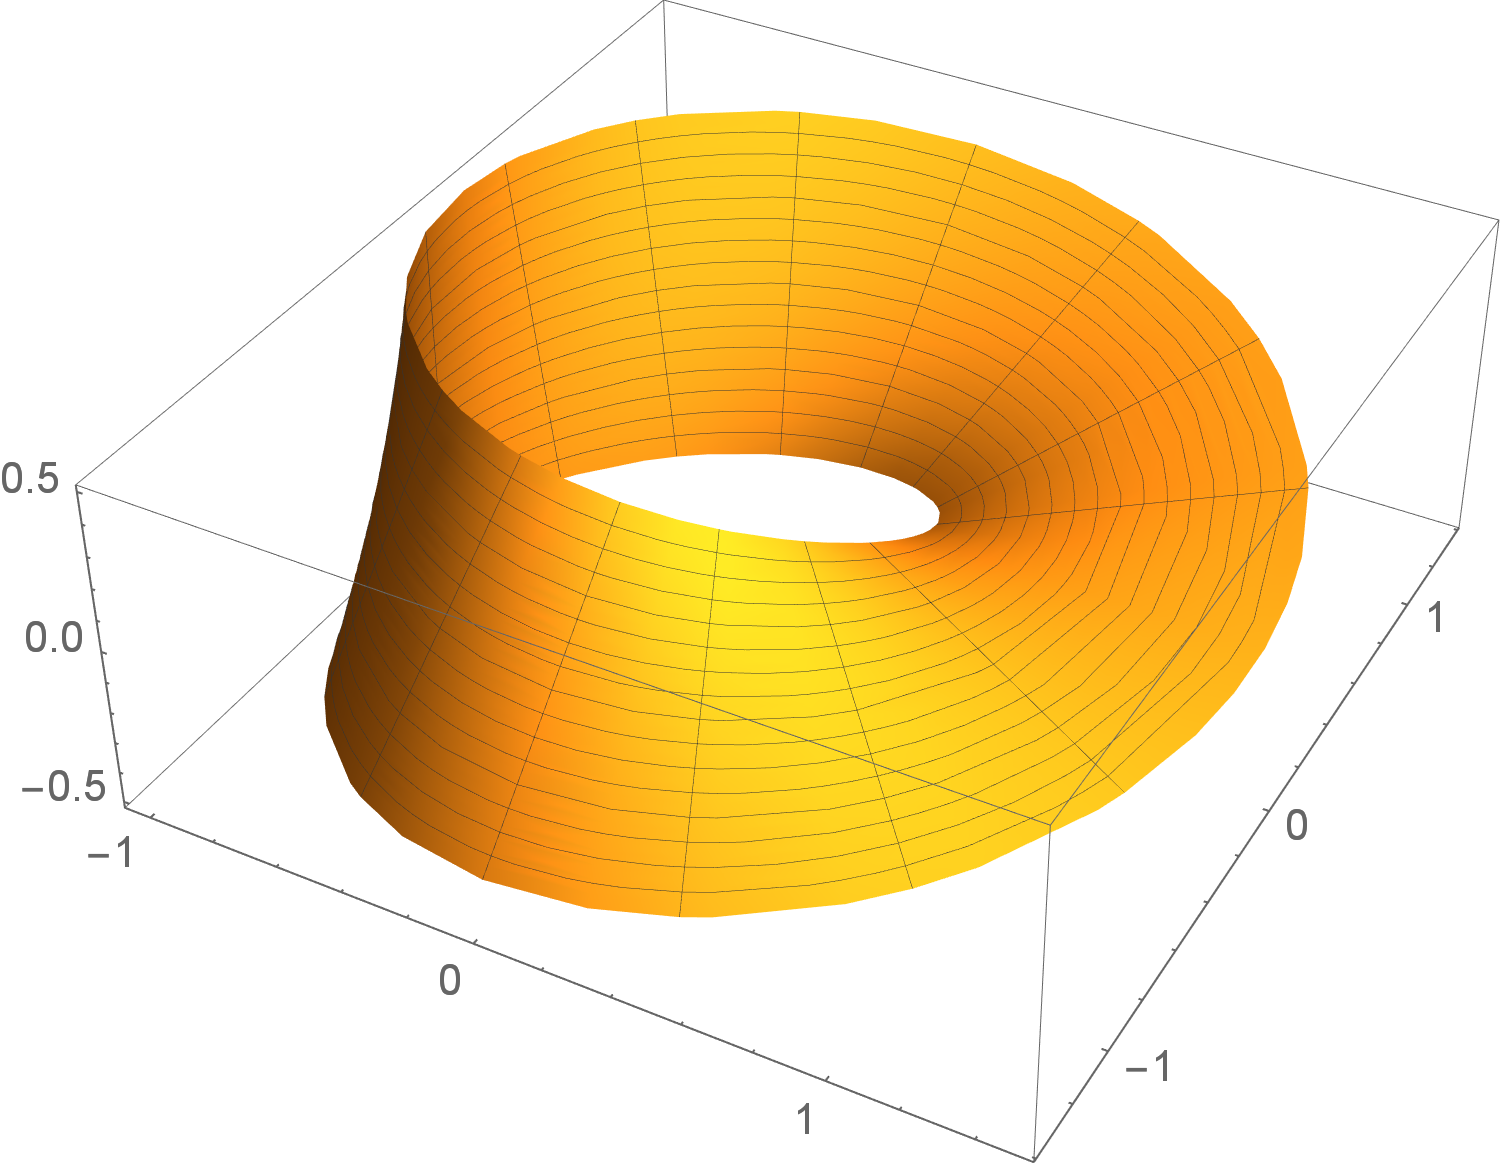
\includegraphics{mobius.png}
\end{image}
This surface is called a \link[M\"{o}bius
  strip]{https://en.wikipedia.org/wiki/Mobius_strip}. It is a
one-sided surface, meaning one could walk along each side of the
surface \textit{without} crossing the edge! M\"obius strips are really
cool, and this author invites you, the young mathematician, to
explore their mysteries on your own.


If you have a closed surface, the normal vector pointing outward
indicates the ``positive'' direction, and the normal vector pointing
inward indicates the ``negative'' direction.  Moreover, given any
parameterization of an orientable surface, there is a natural
orientation based on the parameterization.

\begin{definition}
  Given a parameterization of an orientable surface:
  \[
  \vec{P}(u,v) = \vector{x(u,v), y(u,v), z(u,v)}
  \]
  the \dfn{orientation given by the parameterization} is given by the
  direction of
  \[
  \pp[\vec{P}]{u} \cross\pp[\vec{P}]{v}.
  \]
\end{definition}

Now we have all the ``parts'' of a surface integral, it is time to
explain what they are.





\section{Surface integrals}

To compute the flow across a surface, also known as flux, we'll use a
\textit{surface integral}.  While line integrals allow us to integrate a
vector field $\vec{F}:\R^2\to\R^2$ along a curve $C$ that is
parameterized by $\vec{p}(t) = \vector{x(t),y(t)}$:
\[
\int_C \vec{F}\dotp\d\vec{p}
\]
A \textit{surface integral} allows us to integrate a vector field
$\vec{F}:\R^3 \to \R^3$ across a surface $S$ that is parameterized by
\[
\vec{P}(u,v) =\vector{x(u,v), y(u,v), z(u,v)}.
\]
Consider a patch of a surface $\d S$ along with a unit vector normal
to the surface $\uvec{n}$:
\begin{image}
  \begin{tikzpicture}
    \begin{axis}%
      [width=175pt,height=200pt,
        tick label style={font=\scriptsize},%axis on top,
	axis lines=center,
	view={110}{25},
	name=myplot,
	xtick=\empty,
	ytick=\empty,
	ztick=\empty,
	minor xtick=1,
	minor ytick=1,
	ymin=0,ymax=.5,
	xmin=.6,xmax=1.2,
	zmin=1, zmax=3.1,
        every axis x label/.style={at={(axis cs: .65,-.2,0)}},%,xshift=-1pt,yshift=-1pt},
	xlabel={\scriptsize $x$},
	every axis y label/.style={at={(axis cs:0,.35,0)}},%,xshift=1pt,yshift=-1pt},
	ylabel={\scriptsize $y$},
	every axis z label/.style={at={(axis cs:0,-.18,2.2)}},
	zlabel={\scriptsize $z$},
        colormap/cool
      ]      
      \addplot3[domain=0:1.4,,y domain=0:.4,mesh,samples=15,samples y=9,very thin,z buffer=sort] {-.5*(x-1)^2-.5*(y)^2+2};
      
      %\addplot3[draw=mapped color!0!black,,domain=.8:1,surf,y domain=.2:.3,samples=2,samples y=2, very thick,z buffer=sort] {1.96375+.1*(x-.9)-.25*(y-.25)};
      \addplot3[surf,faceted color=black,,domain=.8:1,y domain=.2:.3,samples=2,samples y=2, ultra thick,z buffer=sort] {1.96375+.1*(x-.9)-.25*(y-.25)};
      
      
      %\draw [penColor,very thick] (axis cs: .8,.2,1) -- (axis cs: .8,.3,1) -- node [pos=.5,right,black] {\scriptsize $\d x$} (axis cs: 1,.3,1) --node [pos=.5,below,black] {\scriptsize $\d y$}(axis cs: 1,.2,1) --(axis cs: .8,.2,1)--(axis cs: .8,.3,1);

      \draw (axis cs: .9,.33,1.95) node {\scriptsize $\d S$};
      %(axis cs: 1.1,.27,2) node {\scriptsize $\vec v$};

      \draw[->,ultra thick] (axis cs: .9,.25,1.96375) -- %node {\scriptsize $\uvec n$}
      (axis cs: .9,.25,2.6);

      \node[left] at (axis cs: .9,.25,2.26) {\scriptsize $\uvec n$};
      
      
    \end{axis}
\end{tikzpicture}
\end{image}
A surface integral will use the dot product to see how ``aligned''
field vectors are with this (scaled) unit normal vector.
\begin{definition}
Let $\vec{F}:\R^3\to\R^3$ be a vector field and $\vec{P}:\R^2\to\R^3$
be a smooth vector-valued function drawing an oriented surface $S$ exactly once
as $u$ runs from $a$ to $b$ and $v$ runs from $c$ to $d$:
\begin{align*}
  \vec{F}(x,y,z) &= \vector{L(x,y,z), M(x,y,z), N(x,y,z)}\\
  \vec{P}(u,v) &= \vector{x(u,v),y(u,v),z(u,v)}.
\end{align*}
A \dfn{surface integral} is an integral of the form:
\begin{align*}
  \iint_R \vec{F}\dotp \uvec{n} \d S &= \int_c^d\int_a^b \vector{L,M,N}
  \dotp \frac{\left(\pp[\vec{P}]{u}\cross\pp[\vec{P}]{v}\right)}{\left|\pp[\vec{P}]{u}\cross\pp[\vec{P}]{v}\right|}\left|\pp[\vec{P}]{u}\cross\pp[\vec{P}]{v}\right|\d u \d v\\
  &= \int_c^d\int_a^b \vector{L,M,N}
  \dotp \left(\pp[\vec{P}]{u}\cross\pp[\vec{P}]{v}\right)\d u \d v
\end{align*}
\end{definition}

\begin{question}
  Consider a surface integral:
  \[
  \iint_R \vec{F}\dotp \uvec{n} \d S
  \]
  Suppose that $\vec{P}(x,y) = \vector{x,y,G(x,y)}$ for $a\le x\le b$
  and $c\le y\le d$. Simplify the integral above.
  \begin{prompt}
    \[
    \iint_R \vec{F}\dotp \vector{-\pp[\answer{G}]{\answer{x}}, -\pp[\answer{G}]{\answer{y}},\answer{1}}\d A
    \]
  \end{prompt}
\end{question}

Now let's work some examples.

\begin{example}
  Consider the vector field $\vec{F}$ and the surface $\vec{P}$
  \begin{align*}
    \vec{F}(x,y,z) &= \vector{y-z,x-z,x-y}\\
    \vec{P}(s,t) &= \vector{s-t,t-s,2t+s}
  \end{align*}
  for $0\le s\le 1$ and $1-s\le t\le 1$.  Using the orientation given
  by the parameterization of $\vec{P}$, compute:
  \[
  \iint_R \vec{F}\dotp \uvec{n}\d S
  \]
  \begin{explanation}
    First we'll compute $\uvec{n}\d S$. We know that
    \begin{align*}
      \uvec{n}\d S &= \left(\pp[\vec{P}]{\answer[given]{s}}\cross\pp[\vec{P}]{\answer[given]{t}}\right)\d t \d s\\
      &=\left(
      \vector{\answer[given]{1},\answer[given]{-1},\answer[given]{1}}
      \cross
      \vector{\answer[given]{-1},\answer[given]{1},\answer[given]{2}}
      \right)\d t \d s\\
       &=
      \vector{\answer[given]{-3},\answer[given]{-3},\answer[given]{0}}
      \d t \d s.
    \end{align*}
    Now write:
    \[
    \vec{F}(\vec{P}(s,t)) = \vector{\answer[given]{-2s-t},\answer[given]{-3t},\answer[given]{2s-2t}}
    \]
    So, write with me,
    \begin{align*}
      \iint_R \vec{F}\dotp \uvec{n}\d S &=
      \int_{\answer[given]{0}}^{\answer[given]{1}}\int_{\answer[given]{1-s}}^{\answer[given]{1}} \left(\answer[given]{6s + 12 t}\right)\d t \d s\\
      &=
      \int_{\answer[given]{0}}^{\answer[given]{1}}\answer[given]{12s} \d s\\
      &=\answer[given]{6}.
    \end{align*}
  \end{explanation}
\end{example}

\begin{example}
  Consider the vector field $\vec{F}$ and the surface $\vec{P}$
  \begin{align*}
    \vec{F}(x,y,z) &= \vector{x,y,z}\\
    \vec{P}(\theta,\phi) &= \vector{\cos(\theta)\sin(\phi),\sin(\theta)\sin(\phi),\cos(\phi)}
  \end{align*}
  for $0\le \theta<2\pi$ and $0\le \phi\le \pi$.  Using the outward
  pointing orientation, compute:
  \[
  \iint_R \vec{F}\dotp \uvec{n}\d S
  \]
  \begin{explanation}
    First we'll compute $\uvec{n}\d S$, paying attention to the
    orientation. We know that
    \begin{align*}
      \uvec{n}\d S &= \left(\pp[\vec{P}]{\answer[given]{\theta}}\cross\pp[\vec{P}]{\answer[given]{\phi}}\right)\d\phi\d\theta\\
      &=\begin{bmatrix}
      \answer[given]{-\sin(\theta)\sin(\phi)}\\
      \answer[given]{\cos(\theta)\sin(\phi)}\\
      \answer[given]{0}
      \end{bmatrix}
      \cross
      \begin{bmatrix}
        \answer[given]{\cos(\theta)\cos(\phi)}\\
        \answer[given]{\sin(\theta)\cos(\phi)}\\
        \answer[given]{-\sin(\phi)}
      \end{bmatrix}
      \d\phi\d\theta\\
       &=
      \begin{bmatrix}
        \answer[given]{-\cos(\theta)\sin^2(\phi)}\\
        \answer[given]{-\sin(\theta)\sin^2(\phi)}\\
        \answer[given]{-\cos(\phi)\sin(\phi)}
      \end{bmatrix}
      \d\phi\d\theta.
    \end{align*}
    Let's now examine our normal vector. If we check at the angles
    $(\theta,\phi) = (0,0)$ or the angles $(\theta,\phi) = (0,\pi)$
    something strange happens, we find the vector
    $\vector{\answer[given]{0},\answer[given]{0},\answer[given]{0}}$. This
    is an unavoidable consequence of the so-called ``\link[Hariy ball
      theorem]{http://en.wikipedia.org/wiki/Hairy_ball_theorem}.'' Regardless,
    since there are only a finite number of isolated ``bad points''
    our computation is unaffected. Checking the orientation at the
    angles $(\theta,\phi) = (0,\pi/2)$, we find the normal vector
    \[
    \vector{-1,0,0}
    \]
    meaning that these normal vectors are oriented
    \wordChoice{\choice[correct]{inward}\choice{outward}}. Hence we will now set
    \[
    \uvec{n}\d S = \vector{\answer[given]{\cos(\theta)\sin^2(\phi)},\answer[given]{\sin(\theta)\sin^2(\phi)},\answer[given]{\cos(\phi)\sin(\phi)}}
      \d\phi\d\theta.
    \]
    Now write:
    \[
    \vec{F}(\vec{P}(\theta,\phi)) = \vector{\answer[given]{\cos(\theta)\sin(\phi)},\answer[given]{\sin(\theta)\sin(\phi)},\answer[given]{\cos(\phi)}}
    \]
    So, write with me,
    \begin{align*}
      \iint_R \vec{F}\dotp \uvec{n}\d S &=
      \int_{\answer[given]{0}}^{\answer[given]{2\pi}}\int_{\answer[given]{0}}^{\answer[given]{\pi}} \left(\answer[given]{\sin(\phi)}\right)\d\phi \d\theta\\
      &=
      \int_{\answer[given]{0}}^{\answer[given]{2\pi}}\answer[given]{2} \d\theta\\
      &=\answer[given]{4\pi}.
    \end{align*}
  \end{explanation}
\end{example}


\begin{example}
  In the first episode of the science fiction series \textit{The
    Expanse}, the \textit{Canterbury} (a space ship hulling water) is
  destroyed. Several ``lucky'' crew members escape destruction in a
  small shuttle $2.6\cdot 10^7$ meters away, only later to be pummeled by
  debris.
  
\begin{center}
  \youtube{AgFT7NQr9ms}%https://www.youtube.com/watch?v=AgFT7NQr9ms
\end{center}

Setting
  \begin{align*}
    \vec{F}(x,y,z) &= \frac{2\cdot 10^5 \vec{x}}{\pi |\vec{x}|^3}\\
    \vec{P}(\theta,\phi) &= 2.6\cdot 10^7\vector{\cos(\theta)\sin(\phi),\sin(\theta)\sin(\phi),\cos(\phi)}
  \end{align*}
  where $\vec{x} = \vector{x,y,z}$, $0\le\theta<2\pi$, and $0\le
  \phi\le 4\cdot 10^{-7}$ the surface integral
  \[
  \iint_R \vec{F}\dotp \uvec{n}\d S
  \]
  will compute the momentum (in kilograms per second) that will
  impact the shuttle in kilograms-per-second. Find this value.
  \begin{explanation}
    From our work above we know that
    \[
    \uvec{n}\d S = 6.76\cdot 10^{14} \vector{\answer[given]{\cos(\theta)\sin^2(\phi)},\answer[given]{\sin(\theta)\sin^2(\phi)},\answer[given]{\cos(\phi)\sin(\phi)}}
    \d\phi\d\theta.
    \]
    Now write:
    \[
    \vec{F}(\vec{P}(\theta,\phi)) = \answer[given]{\frac{1}{3.38\cdot10^{9}\pi}}\vector{\cos(\theta)\sin(\phi),\sin(\theta)\sin(\phi),\cos(\phi)}
    \]
    So, write with me,
    \begin{align*}
      \iint_R \vec{F}\dotp \uvec{n}\d S &=
      \frac{2\cdot 10^5}{\pi}\int_{\answer[given]{0}}^{\answer[given]{2\pi}}\int_{\answer[given]{0}}^{\answer[given]{4\cdot 10^{-7}}} \left(\answer[given]{\sin(\phi)}\right)\d\phi \d\theta\\
      &=4\cdot 10^5 \left(\cos\left(\frac{1}{2.5\cdot 10^6}\right)-1\right)\\
      &\approx 3.2\cdot 10^{-8}.
    \end{align*}
    Hence it is likely no harm would come from the debris.
  \end{explanation}
\end{example}

For some interesting extra reading check out:
\begin{itemize}
\item \link[\textit{Using Differentials to Bridge the Vector Calculus Gap}, J.\ Dray and C.A.\ Manogue, College Math Journal, September
  2003.]{http://www.jstor.org/stable/3595765}
\end{itemize}


\end{document}
